\section{Supersymmetry}
\label{sec:susy}

\begin{align}
    Q \ket{\text{fermion}} = \ket{\text{boson}}, \hspace{1cm} Q \ket{\text{boson}} = \ket{\text{fermion}}
    \label{eq:susy_operator}
\end{align}

\begin{align}
    \left( \Delta m_h^2 \right)_{S} = \frac{\lambda_S}{16 \pi^2} \left[ 2 \Lambda^2 - \mathcal{O} \left( m_S^2 \ln \left( \frac{\Lambda}{m_S} \right) \right) \right]
    \label{eq:higgs_corr_susy}
\end{align}

\begin{align}
    \Delta m_h^2 \underset{\text{w/ SUSY}}{\propto} \left( m_f^2 - m_S^2 \right) \ln \left( \frac{\Lambda}{m_S} \right) + 3 m_f^2 \ln \left( \frac{m_S}{m_f} \right) + \mathcal{O} \left( \frac{1}{\Lambda^2} \right)
    \label{eq:higgs_corr_fixed}
\end{align}

\begin{table}[!htb]
    \begin{center}
        \caption{
            Particle content of the MSSM.
        }
        \label{tab:mssm_particles}
        \begin{tabular}{c | c | c | Sc | Sc}
        \hline
        \hline
            \textbf{Names} & \textbf{Spin} & \textbf{R-Parity} & \textbf{Gauge Eigenstate} & \textbf{Mass Eigenstate} \\
            \hline
            \multirow{3}{*}{Squarks} & \multirow{3}{*}{0} & \multirow{3}{*}{$-1$} & $\tilde{u}_L, \,\tilde{u}_R, \, \tilde{d}_L, \, \tilde{d}_R$ & same  \\
                                                & & & $\tilde{c}_L, \,\tilde{c}_R, \, \tilde{s}_L, \, \tilde{s}_R$ & same  \\
                                                & & & $\tilde{t}_L, \,\tilde{t}_R, \, \tilde{b}_L, \, \tilde{b}_R$ & $\tilde{t}_1,\,\tilde{t}_2,\,\tilde{b}_1,\,\tilde{b}_2$  \\
            \hline
            \multirow{3}{*}{Sleptons} & \multirow{3}{*}{0} & \multirow{3}{*}{$-1$} & $\tilde{e}_L,\,\tilde{e}_R,\,\tilde{\nu}_e$ & same \\
                & & & $\tilde{\mu}_L,\,\tilde{\mu}_R,\,\tilde{\nu}_{\mu}$ & same \\
                & & & $\tilde{\tau}_L,\,\tilde{\tau}_R,\,\tilde{\nu}_{\tau}$ & $\tilde{\tau}_1,\,\tilde{\tau}_2,\,\tilde{\nu}_{\tau}$ \\
            \hline
            Neutralinos & $1/2$ & $-1$ & $\tilde{B}^0,\,\tilde{W}^0,\,\tilde{H}^0_u,\,\tilde{H}^0_d$ & $\tilde{\chi}^0_1,\,\tilde{\chi}^0_2,\,\tilde{\chi}^0_3,\,\tilde{\chi}^0_4$ \\
            \hline
            Charginos & $1/2$ & $-1$ & $\tilde{W}^{\pm},\,\tilde{H}^+_u,\,\tilde{H}^-_d$ & $\tilde{\chi}^{\pm}_1,\,\tilde{\chi}^{\pm}_2$ \\
            \hline
            Gluino & $1/2$ & $-1$ & $\tilde{g}$ & same \\
            \hline
            \hline
            Higgs Bosons & 0 & $+1$ & $H_u^0,\,H_d^0,\,H_u^+,\,H_d^-$ & $h^0,\,H^0,\,A^0,\,H^{\pm}$  \\
        \hline
        \hline
        \end{tabular}
    \end{center}
\end{table}

\begin{align}
    \underbrace{\begin{pmatrix}
        f_{\small{1/2}} \\
        \tilde{\phi}_0
    \end{pmatrix}}_{\substack{\text{Chiral} \\ \text{Supermultiplet}}}
    \hspace{1cm}
    \underbrace{\begin{pmatrix}
        V_1 \\
        \tilde{V}_{1/2}
    \end{pmatrix}}_{\substack{\text{Gauge} \\ \text{Supermultiplet}}}
    \hspace{1cm}
    \begin{matrix}
        \begin{cases}
            \begin{tabular}{l l}
                $f_{1/2}$~: & \text{Spin-1/2 Weyl fermion} \\
                $\tilde{\phi}_0$~: & \text{Complex scalar} 
            \end{tabular}
        \end{cases} \\
        %\hspace{1.3cm}
        \begin{cases}
            \begin{tabular}{l l}
                $V_1$~: & \text{Spin-1 boson} \\
                $\tilde{V}_{1/2}$~: & \text{Spin-1/2 Weyl fermion}
            \end{tabular}
        \end{cases}
    \end{matrix}
    \label{eq:susy_multiplets}
\end{align}

%\begin{align}
%    \rho = \frac{
%                M_W
%            }
%            {
%                M_Z \cos \theta_W
%            }
%        \underset{\text{\tiny{SM}}}{=} 1
%    \label{eq:rho_sm}
%\end{align}
%
%\begin{align}
%    \rho = \frac{
%                \sum\limits_{i = 1}^n \, \left[ T_{3,i} \left( T_{3,i} + 1 \right) - \frac{1}{2} Y_i^2 \right ] v_i
%            }
%            {
%                \sum\limits_{i=1}^n \, Y_i^2 v_i
%            }
%    \label{eq:rho_general}
%\end{align}

\begin{figure}[!htb]
    \begin{center}
        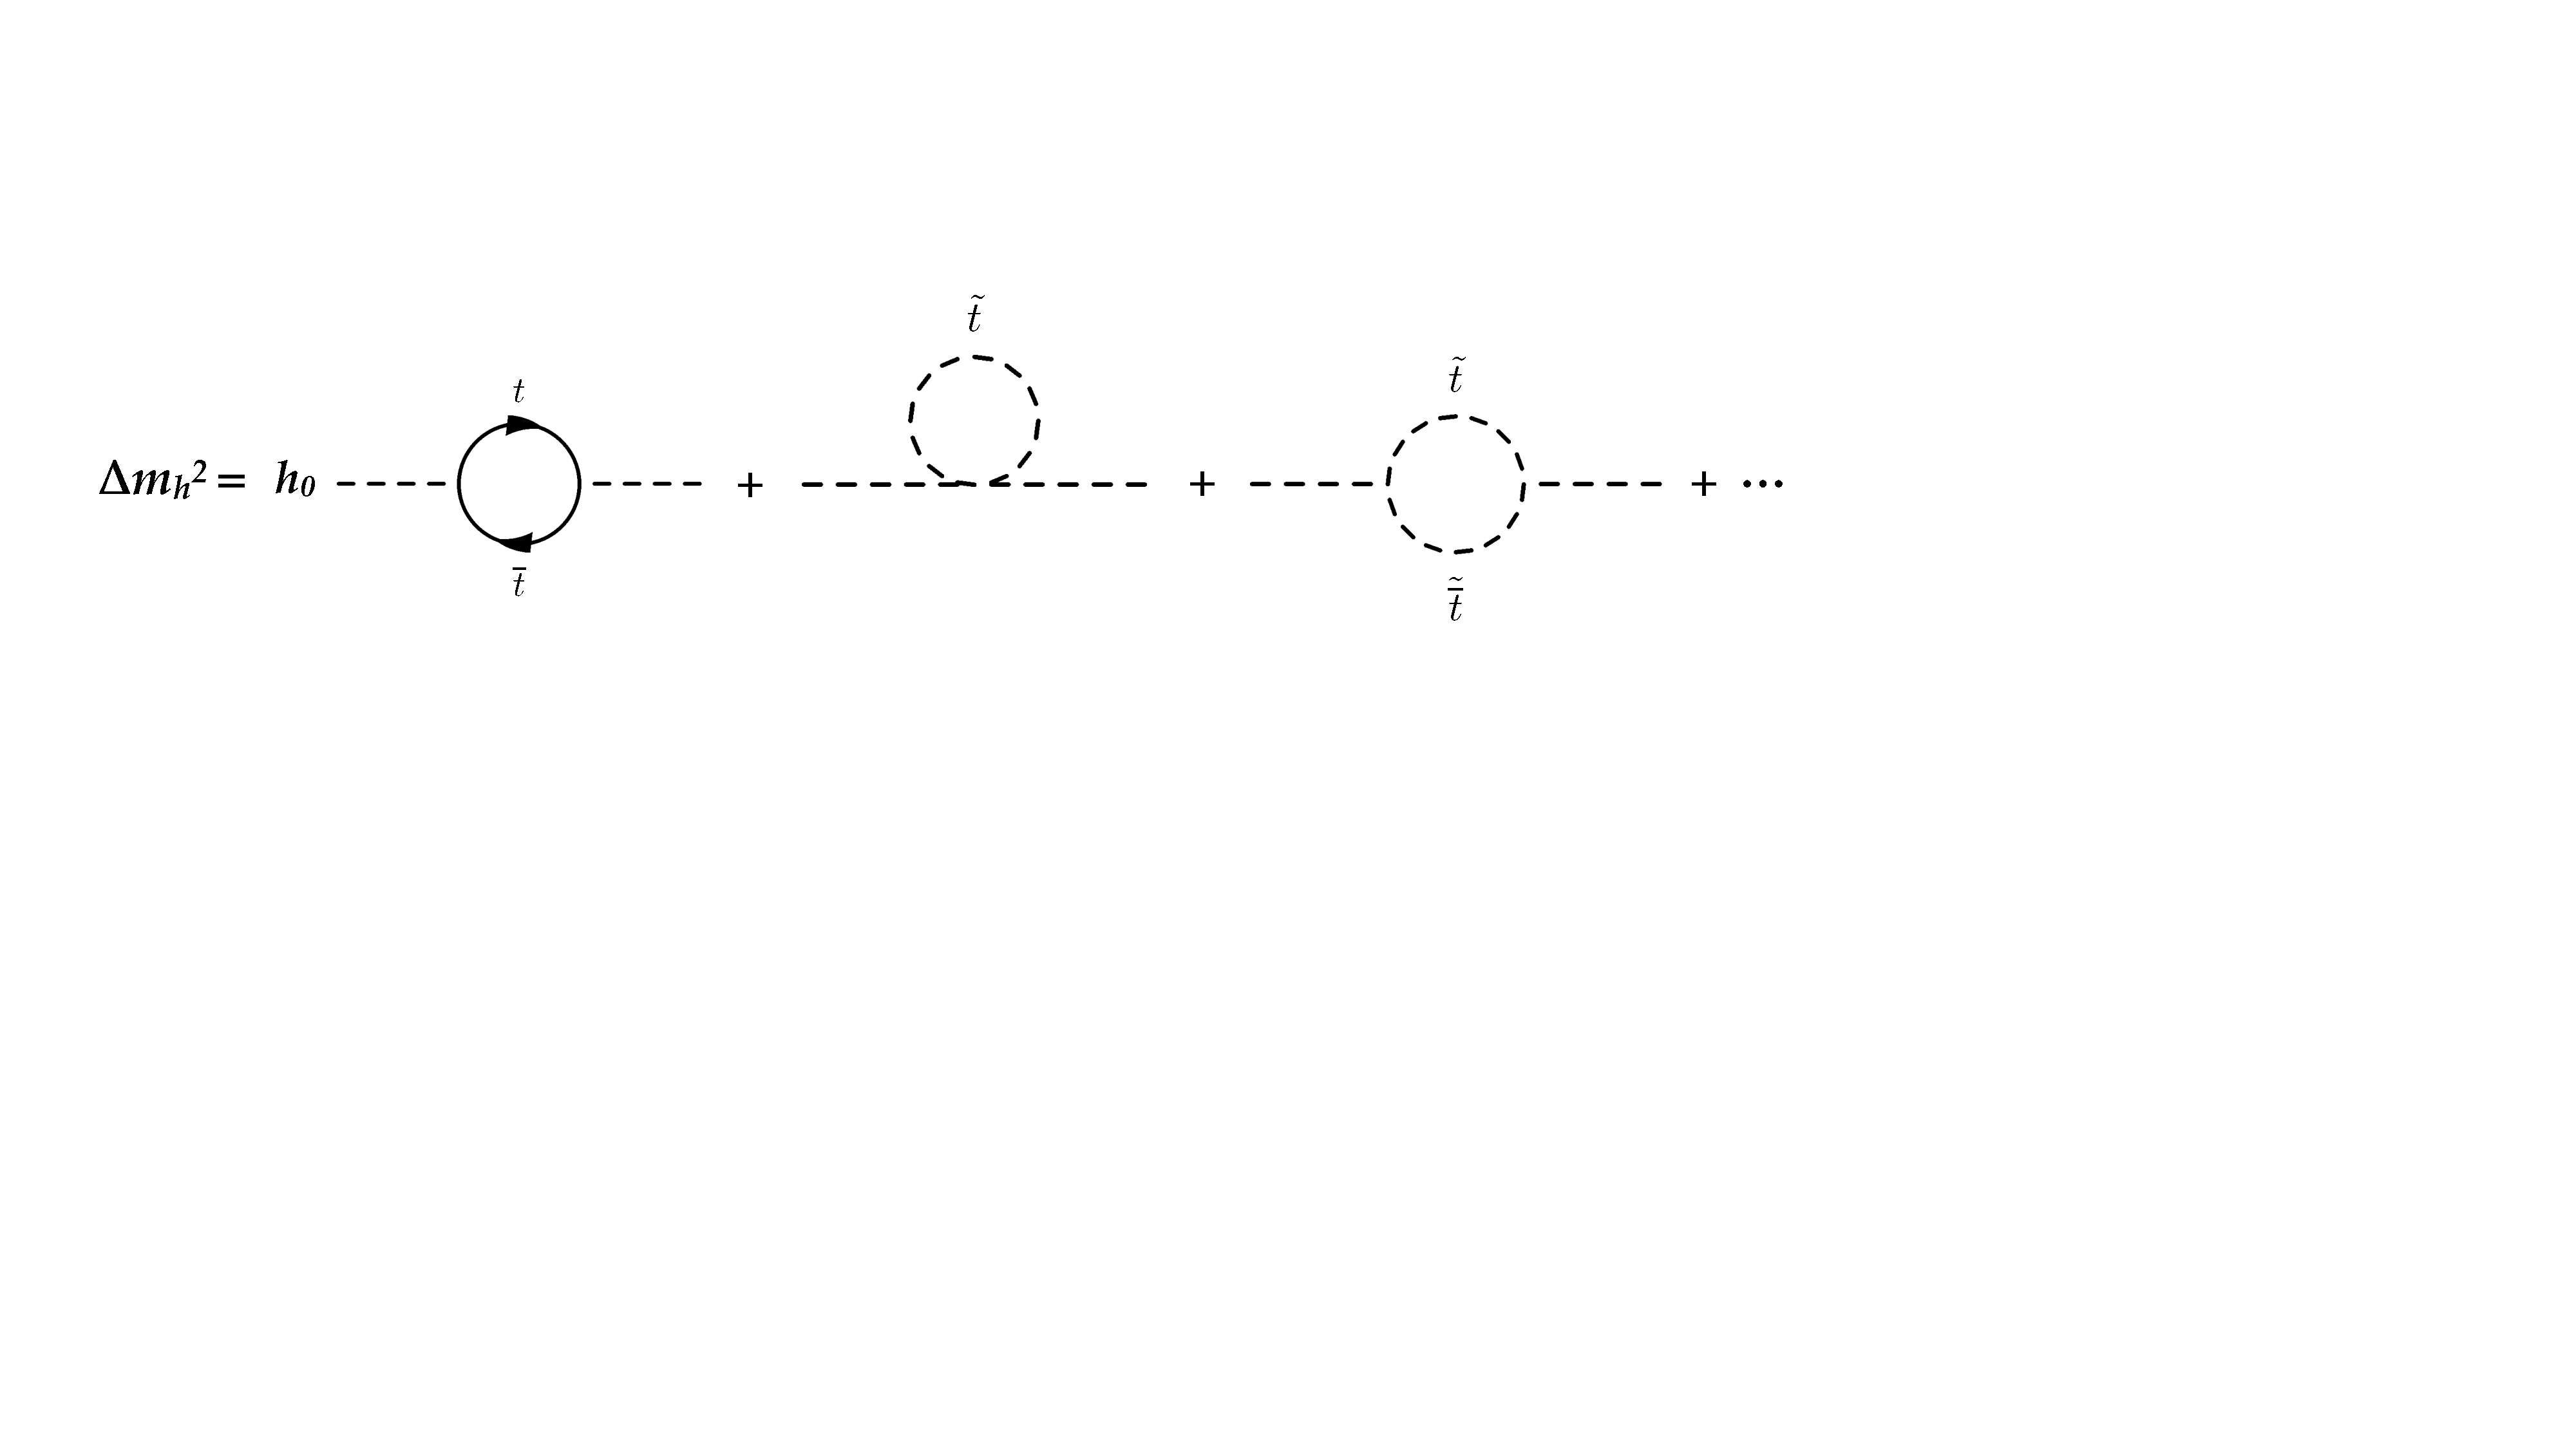
\includegraphics[width=0.9\textwidth]{figures/higgs_corr/higgs_mass_corrections_stopPDF}
        \caption{
            Top and stop-quark loop contributions to the higher-order computation of the
            Higgs mass.
        }
        \label{fig:higgs_mass_correction_stop}
    \end{center}
\end{figure}

\begin{figure}[!htb]
    \begin{center}
        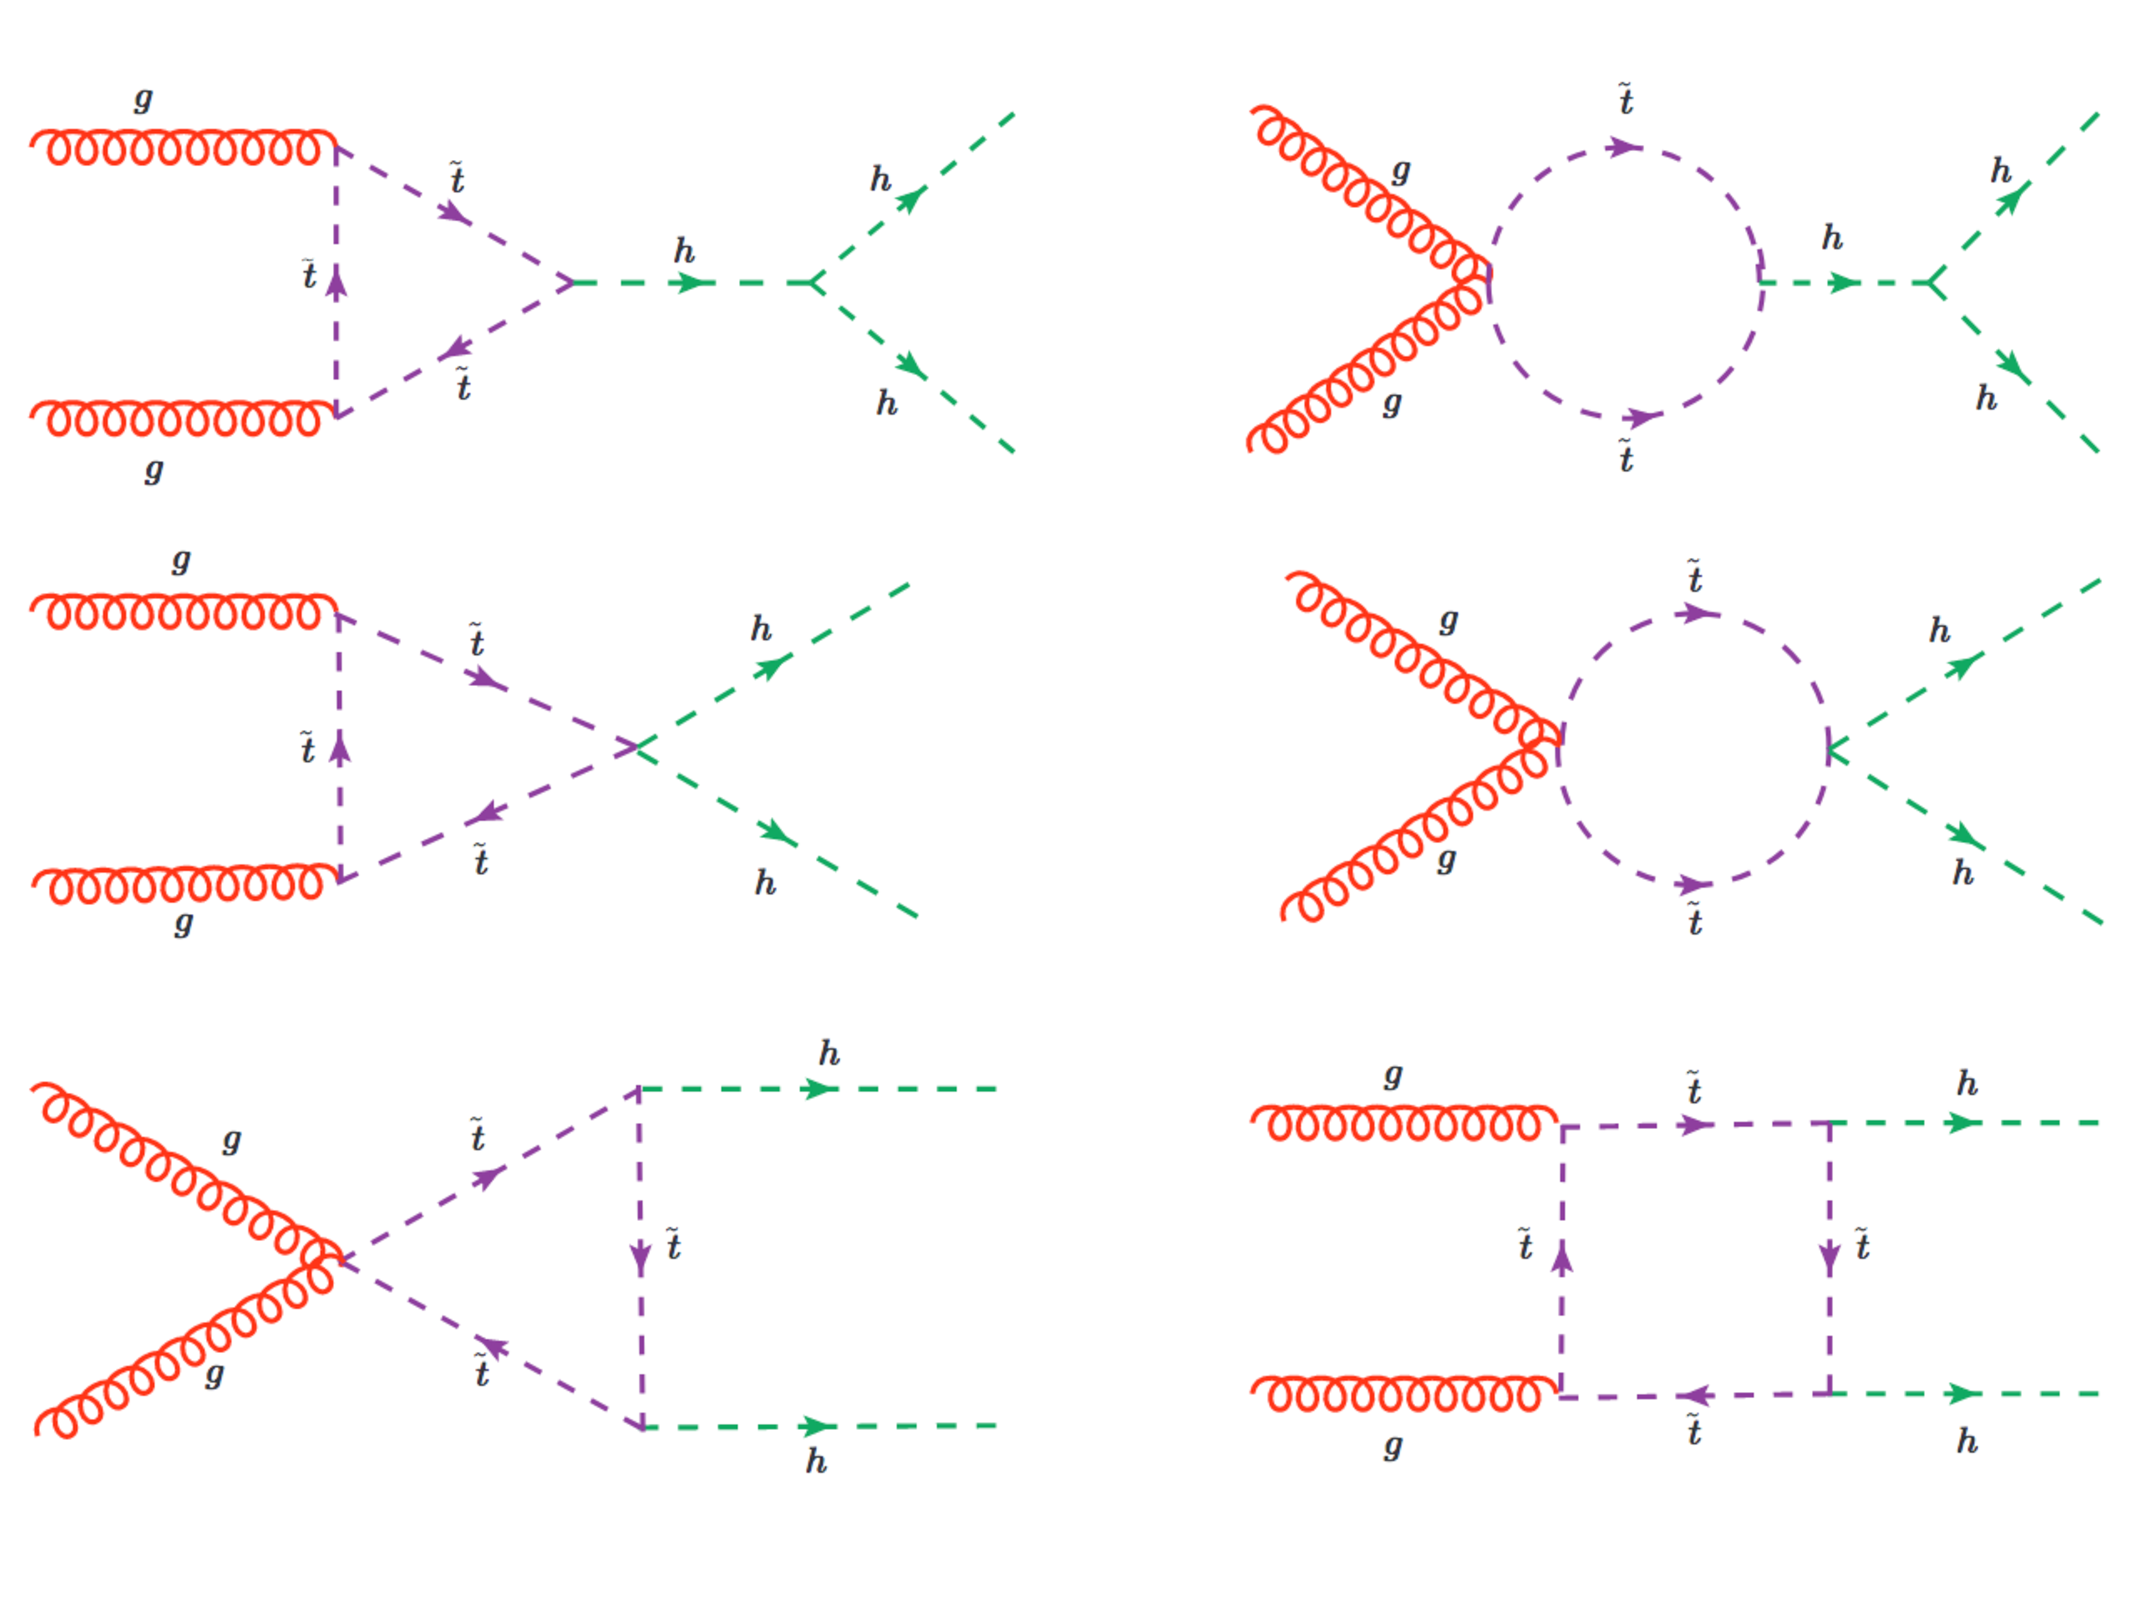
\includegraphics[width=0.95\textwidth]{figures/higgs_corr/hh_stopsPDF}
        \caption{
            Single-loop stop-quark diagrams in the MSSM that contribute to the non-resonant production
            of Higgs boson pair, in addition to those already predicted in the SM (Figure~\ref{fig:hh_feynman}). From Ref.~\cite{LightStopsHiggs}.
        }
        \label{fig:hh_stops}
    \end{center}
\end{figure}

\begin{figure}[!htb]
    \begin{center}
        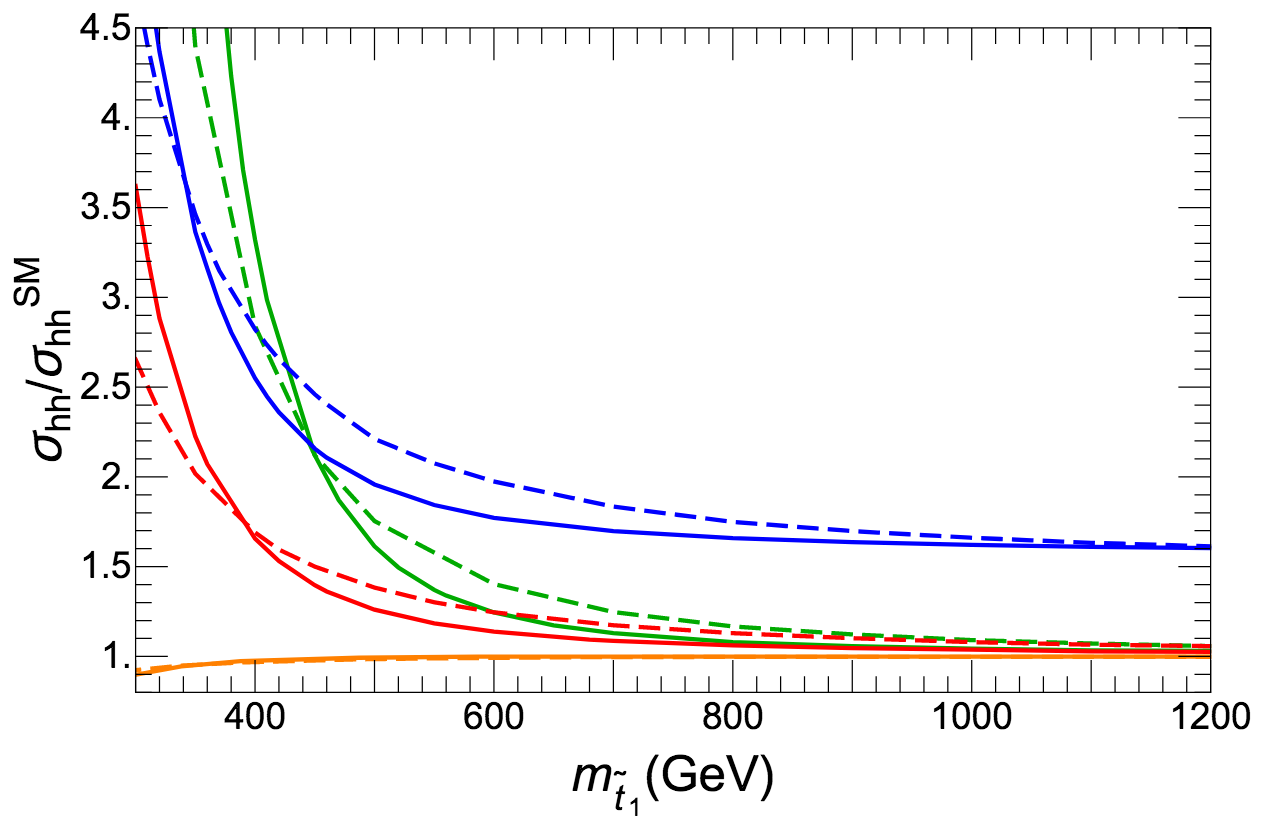
\includegraphics[width=0.65\textwidth]{figures/higgs_corr/sigma_hh_stops}
        \caption{
            Higgs pair production cross-section normalized to the SM prediction as a function
            of the mass of the lighter stop quark, $\tilde{t}_1$.
            Details in Ref.~\cite{LightStopsHiggs}.
        }
        \label{fig:hh_sigma_stops}
    \end{center}
\end{figure}
